\documentclass[../../main.tex]{subfiles}

\begin{document}

\subsection{Motivation}

The aim of lab is use a generalized multilinear regression model, termed the Higher-Order Partial Least Squares (HOPLS) \cite{zhao2012higher}, to predict a tensor $\underline{Y}$ from a tensor $\underline{X}$ through projecting the data onto the latent space and performing regression on the corresponding latent variables. Specifically, We have problem of recognition human body position. On video with person we need to mark the position of the main points of the body (face, shoulders, hips, elbows, lap, ankle). The experiment is carried out on JHMDB (Joint-annotated Human Motion Data Base) \cite{Jhuang:ICCV:2013}.

\subsection{Problem statement}

Given video with person and skeleton's coordinates for each frame of this video:
\[
\label{eq:example:1}
\begin{aligned}
    \mathfrak{D} = \left\{\underline{X_i}, ~\underline{Y_i}\right\}_{i=1}^{K},
\end{aligned}
\]
where ~$\underline{X_i} \in \mathbb{R}^{T \times W\times H\times C}, ~\underline{Y_i} \in \mathbb{R}^{T \times D \times I}$,\\ 
~$T$ - number of framres,  ~{W} - width, ~{H} - height, ~{C} - channel,\\ ~{I} - number of points in skeleton, ~{D} - picture dimension.\\
\\
In our case, $T \leqslant 40, ~W = 320, ~H = 240, ~C = 3, ~I = 15, ~D = 2.$\\
\\
The n-mode product of a tensor
$ X \in \mathbb{R}^{I_1\times ... \times I_n \times ... \times I_N}$
and matrix $A \in \mathbb{R}^{J_n\times I_n}$
is denoted by $\underline{Y} = \underline{X} \times_{i}A \in \mathbb{R}^{I_1\times ... \times I_{n-1} \times J_n \times I_{n+1} \times ... \times I_N}$
and defined as:
$$y_{i_1...i_{n-1}j_ni_{n+1}...i_N } = \sum_{i_n} x_{i_1...i_n...i_N }a_{j_ni_n}$$
$$\underline{Y} = \underline{G} \times_{1} A^{(1)} \times_{2} A^{(2)} \times_{3} ...\times_{N} A^{(N)} + \underline{E} = [[G; A^{(1)}, A^{(2)}, ..., A^{(N)}]] + \underline{E}$$

We assume $\underline{X}$ is decomposed as a sum of $rank-(1, L_2, . . . , L_N )$ Tucker blocks, while $\underline{Y}$ is decomposed as a sum of $rank-(1, K_2, . . . , K_M)$ Tucker blocks, which can be expressed as

$$\underline{X} = \sum_{r=1}^{R}\underline{G_r}\times_{1} t_r \times_{2} P^{(1)}_r \times_{3} P^{(2)}_r \times_{4} ...\times_{N} P^{(N-1)}_r + \underline{E}_r$$
$$\underline{Y} = \sum_{r=1}^{R}\underline{D_r}\times_{1} t_r \times_{2} Q^{(1)}_r \times_{3} Q^{(2)}_r \times_{4} ...\times_{N} Q^{(N-1)}_r + \underline{F}_r$$
where R is the number of latent vectors, $t_r \in \mathbb{R}^{I_1}$ is the r-th latent vector $P_r^{n} \in \mathbb{R}^{I_{n+1} \times L_{n+1}}$ and $Q_r^{m} \in \mathbb{R}^{J_{n+1} \times K_{n+1}}$ are loading matrices on mode-n and mode-m respectively, and $\underline{G_r} \in \mathbb{R}^{1 \times L_{2}\times ...\times L_{N}}$ and $\underline{D_r}\in \mathbb{R}^{1 \times K_{2}\times ...\times K_{M}}$ are core tensors.\\
\\
However the Tucker decompositions are not unique due to the permutation, rotation, and scaling issues. To alleviate this problem, additional constraints should be imposed such that the core tensors $\underline{G_r}$ and $\underline{D_r}$ are all-orthogonal, a sequence of loading matrices are column-wise orthonormal, i.e., $P^{(n)T}_rP^{(n)}_r = I$ and $Q^{(n)T}_rQ^{(n)}_r = I$, the latent vector is of length one, i.e. $\|t_r\|_F=1$.\\
\\
The main aim is to reduce Frobeniuses norm of residuals $\underline{E_r}, \underline{F_r}$. With a few propositions the following optimization problems arise

\[
\label{eq:example:2}
\begin{aligned}
   \min_{P^{(n)}, Q^{(m)}} \| [[C; P^{(1)T}, P^{(2)T}, ..., P^{(N-1)T}, Q^{(1)T}, Q^{(2)T}, ..., Q^{(M-1)T}]]\|_F^2,\\
\end{aligned}
\]
$$s.t. ~P^{(n)T}_rP^{(n)}_r = I, ~Q^{(n)T}_rQ^{(n)}_r = I$$
where $\underline{C} = COV_{\{1;1\}}(\underline{X}, \underline{Y})$.\\
Next, we can find latent vector ~$t$ from 
\[
\label{eq:example:2}
\begin{aligned}
    \min_{t}\| \underline{X} - [[\underline{G};t,P^{(1)},P^{(2)}, ...,P^{(N-1)}]]\|_F^2
\end{aligned}
\]
Now we found the first latent decomposition. Next step is repiting it for $\underline{X} = \underline{E_1}, ~\underline{Y} = \underline{F_1}$.
\subsection{Problem solution}
Full algorithm is described in [1]. Now we can find solution:
$${Y}^{(new)_{(1)}} \approx T^{(new)}Q^{*T} = X^{(new)}_{(1)}WQ^{*T}$$
where ~$W$ and ~$Q^*$ have R columns, represented by 
$$w_r = (P_r^{(N-1)}\otimes ...\otimes P_r^{(1)})\underline{G_{r(1)}^+}$$
$$q_r^* = \underline{D_{r(1)}}(Q_r^{(M-1)}\otimes ...\otimes Q_r^{(1)})^T.$$

\subsection{Code analysis}

The code was taken from \cite{zhao2012higher}.

\subsection{Experiment}

The experiment is carried out on JHMDB (Joint-annotated Human Motion Data Base) \cite{Jhuang:ICCV:2013}.
In our case, $T \leqslant 40, ~W = 320, ~H = 240, ~C = 3, ~I = 15, ~D = 2.$\\
The dataset has 928 videos from 21 class.
\\
Define function of similarity of $\underline{Y}^{(true)}$ and $\underline{Y}^{(predict)}$ as
$Q^2$:
$$Q^2 = 1 - \frac{\|\underline{Y}^{(true)} - \underline{Y}^{(predict)}\|_F^2}{\|\underline{Y}^{(true)}\|_F^2}$$
\\
The first experiment. We divided video into train and test part. Train has 32 frames, test has 8 frames. 
\\
\begin{figure}[h!]
\centering

\includegraphics[width=1\textwidth]{figures/fig1}
\caption{Experiment 1. Dependence $Q^2$ on number of latent vectors R.}
\end{figure}
\\
The second experiment. In our dataset we have very similar videos, so we can lear our model on the first and test on the second video. It will show how robust this method.
\\
\begin{figure}[h!]
\centering
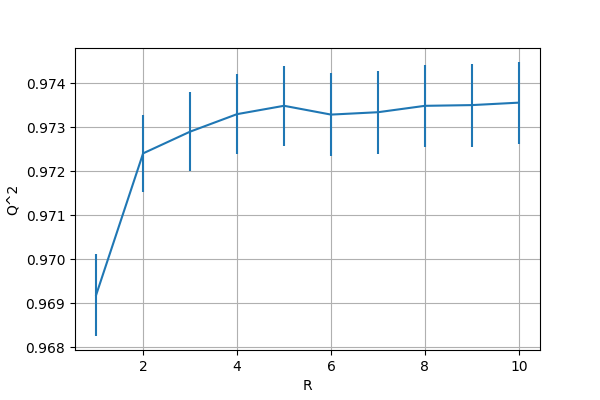
\includegraphics[width=1\textwidth]{figures/fig2}
\caption{Experiment 2. Dependence $Q^2$ on number of latent vectors R.}
\end{figure}

\end{document}